%!TEX root = ../main.tex
%%%%%%%%%%%%%%%%%%%%%%%%%%%%%%%%%%% Links: https://www.yumpu.com/en/document/read/7789379/lowest-common-ancestorlca-chair-for-efficient-algorithms
%
% Difficulty:
% Companies: 
%%%%%%%%%%%%%%%%%%%%%%%%%%%%%%%%%%

\chapter{Distance between nodes in BST}
\label{ch:distance_between_nodes_in_tree}
\section*{Introduction}

\section{Problem statement}
\begin{exercise}
	Write a function that takes as input a binary search tree $T$ and two nodes $p$ and $q$ and returns the distance between $p$ and $q$.
	The distance between two nodes $D(p,q)$ is defined as the number of edges you need to traverse to get from $p$ to $q$.
	
	\begin{example}
		\hfill \\
		Given the tree shown in Figure \ref{fig:distance_between_nodes_in_tree:example1}, 
		$p = 1$ and $q=3$, the function returns $D(1,3)=2$ 
		
		If $p=3$ and $q=2$ the function returna $1$.
	\label{ex:distance_between_nodes_in_tree:example1}
	\end{example}

	\begin{example}
		\hfill \\
		Given the tree shown in Figure \ref{fig:distance_between_nodes_in_tree:example2}, 
		$p = 5$ and $q=2$, the function returns $D(5,2)=6$ 
		\label{ex:distance_between_nodes_in_tree:example2}
	\end{example}
\end{exercise}

\begin{figure}
	\centering
	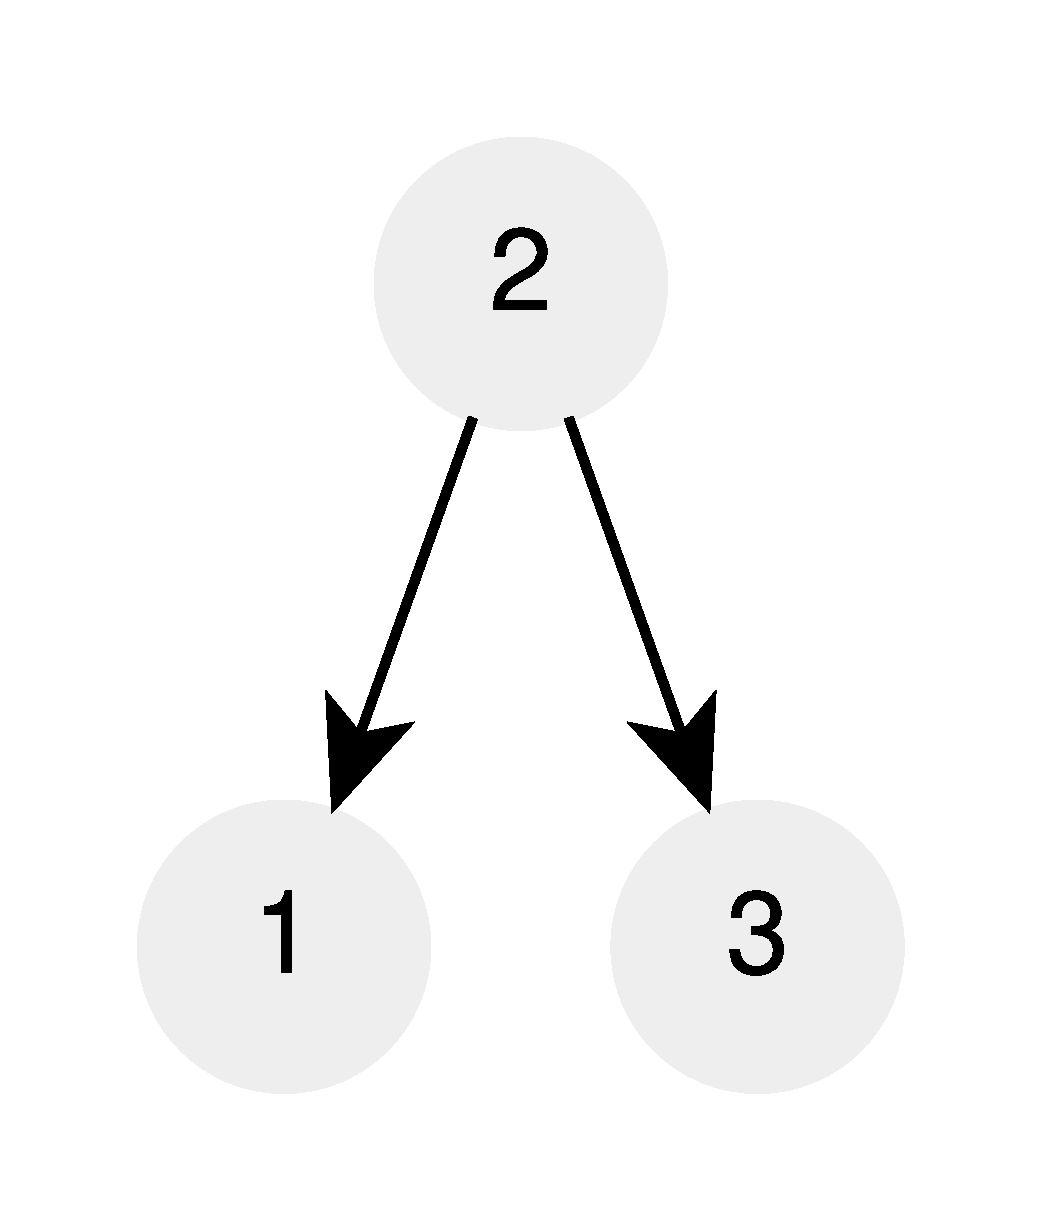
\includegraphics[width=0.3\textwidth]{sources/distance_between_nodes_in_tree/images/example1}
	\caption{Binary Search tree of the Example
	\ref{ex:distance_between_nodes_in_tree:example1}}.
	\label{fig:distance_between_nodes_in_tree:example1}
\end{figure}


\begin{figure}
	\centering
	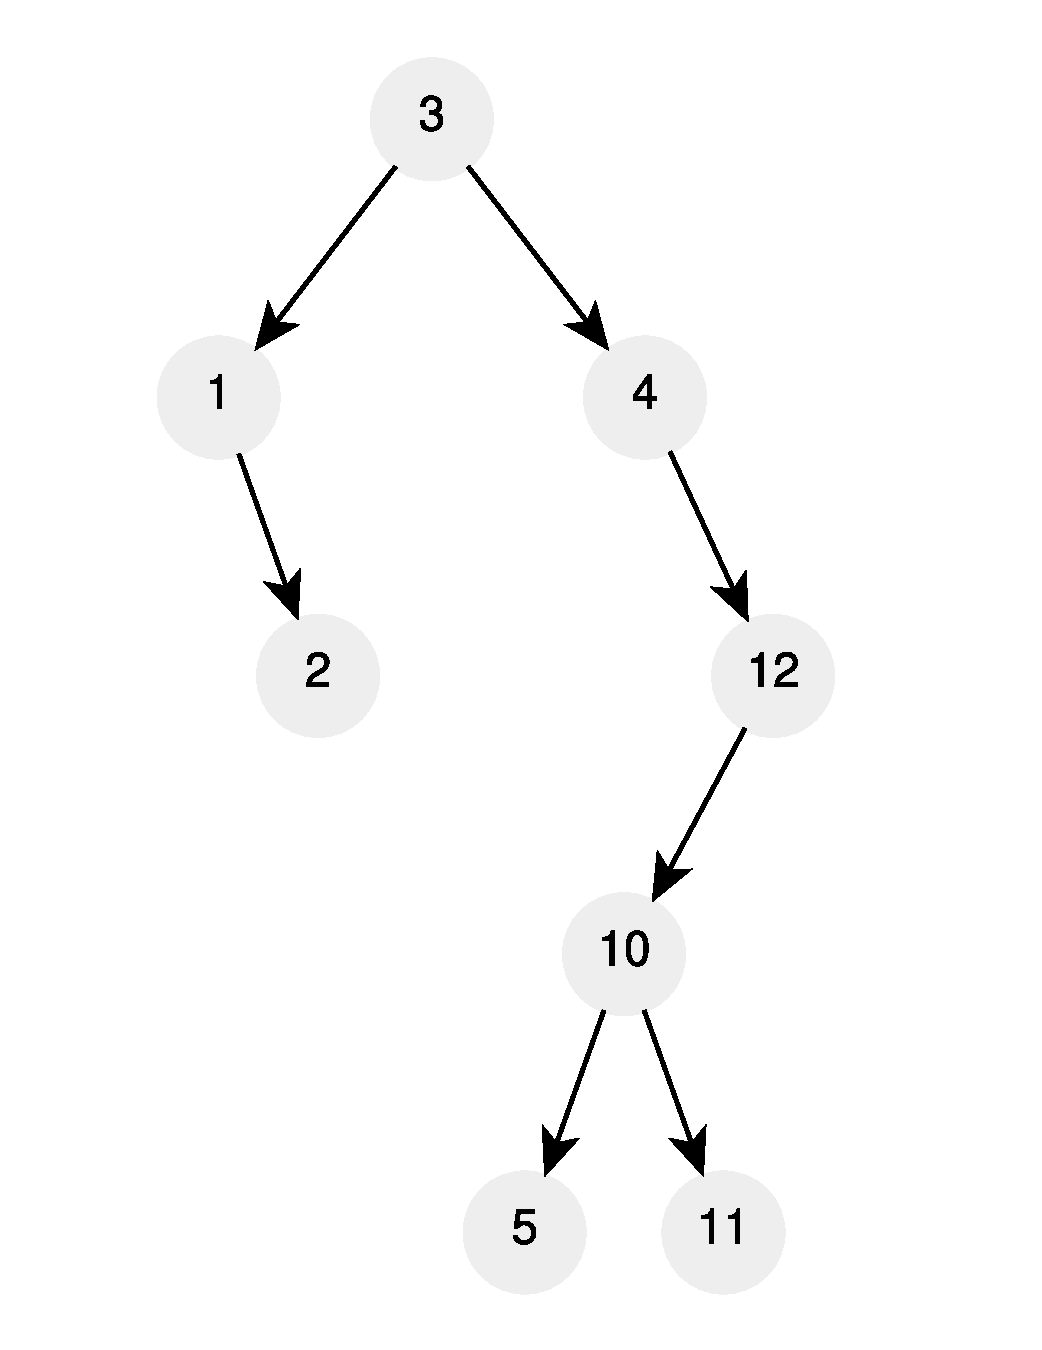
\includegraphics[width=0.5\textwidth]{sources/distance_between_nodes_in_tree/images/example2}
	\caption{Binary Search tree of the Example
	\ref{ex:distance_between_nodes_in_tree:example2}}.
	\label{fig:distance_between_nodes_in_tree:example2}
\end{figure}

\section{Clarification Questions}

\begin{QandA}
	\item Can $p$ be equal to $q$?
	\begin{answered}
		\textit{Yes, this is a valid case.}
	\end{answered}
	
	\item Is it guaranteed for  $p$ and  $q$ to be present in $T$?
	\begin{answered}
		\textit{Yes, you can assume $T$ always contains both $p$ and $q$.}
	\end{answered}

\end{QandA}

\section{Discussion}
\label{distance_between_nodes_in_tree:sec:discussion}

Build BST
Find LCA
Find Distance from LCA to given points
\subsection{Brute-force}
\label{distance_between_nodes_in_tree:sec:bruteforce}

\lstinputlisting[language=c++, caption={Sample Caption},label=list:distance_between_nodes_in_tree]{sources/distance_between_nodes_in_tree/distance_between_nodes_in_tree_solution1.cpp}

